\subsection{Eddy Kinetic Energy and Zonal Mean Zonal Wind}

From Figure \ref{fig:EKE_U_zm_ann} we find:
\begin{itemize}
    \item EKE around 50°S increases in control, together with U ($\pm 5$ m/s), decreases in both SAI scenarios
    \item 
\end{itemize}

\begin{figure}[H]
    \centering
    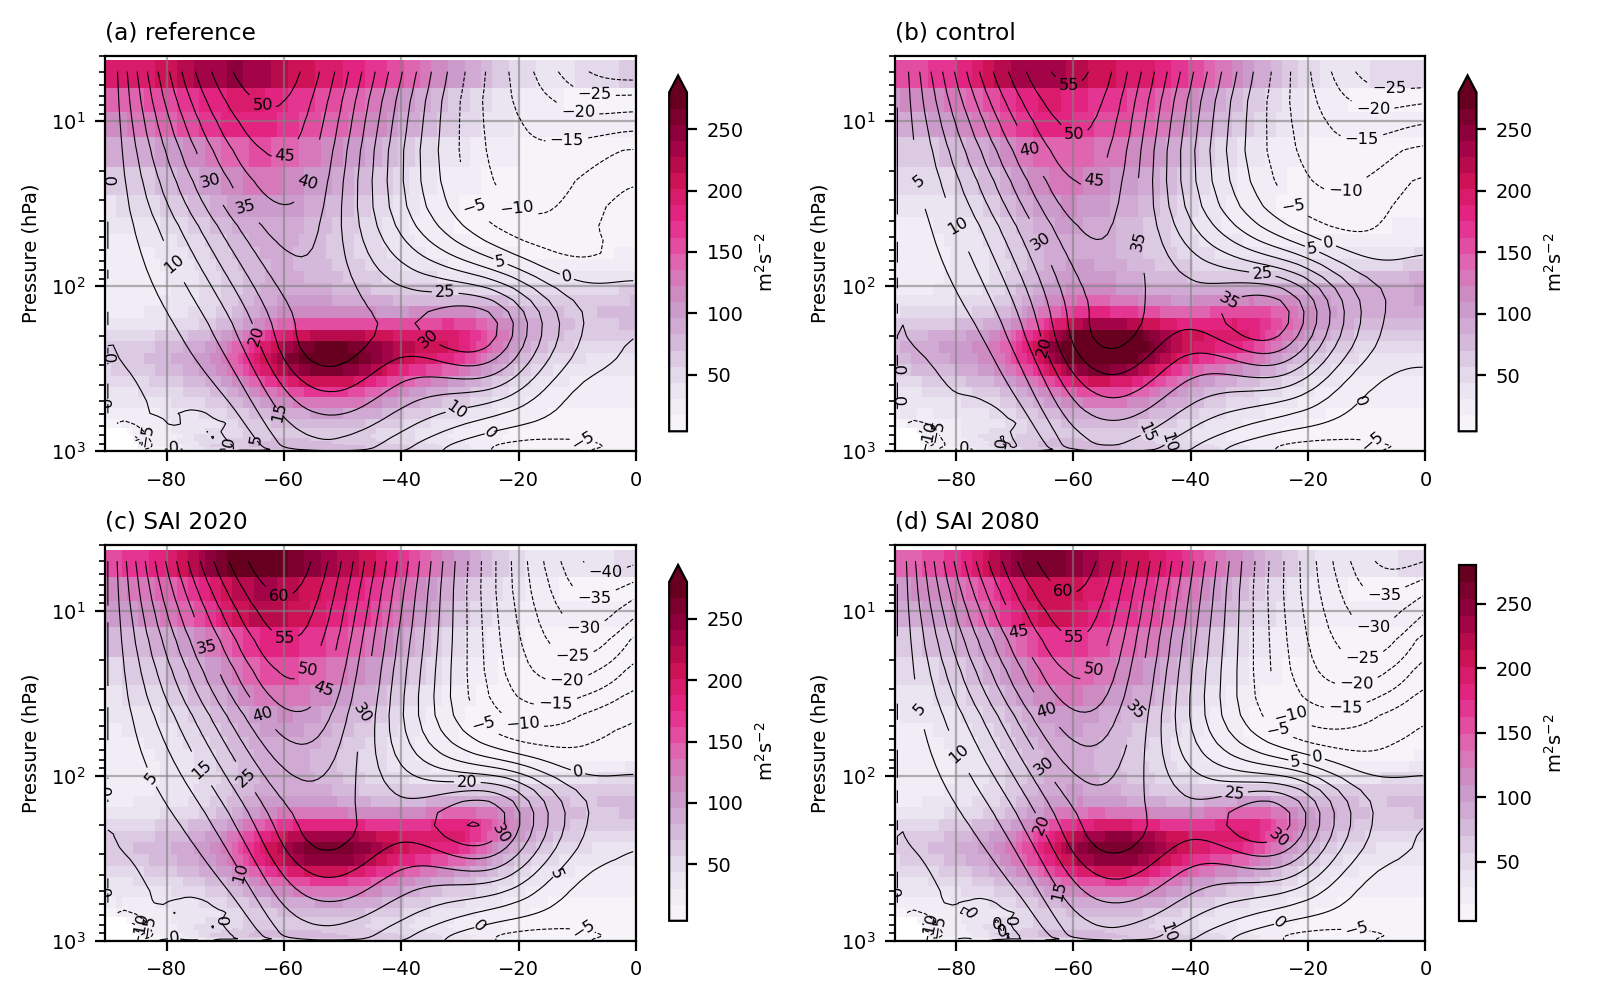
\includegraphics[width=\linewidth]{images/EKE_U_zm_ann.png}
    \caption{Zonal mean EKE in m$^2$/s$^2$ (shading) and zonal mean zonal wind (contours) in intervals of 5 m/s, annual mean for reference 2020-2039 and all scenarios 2111-2130}
    \label{fig:EKE_U_zm_ann}
\end{figure}

\begin{figure}[H]
    \centering
    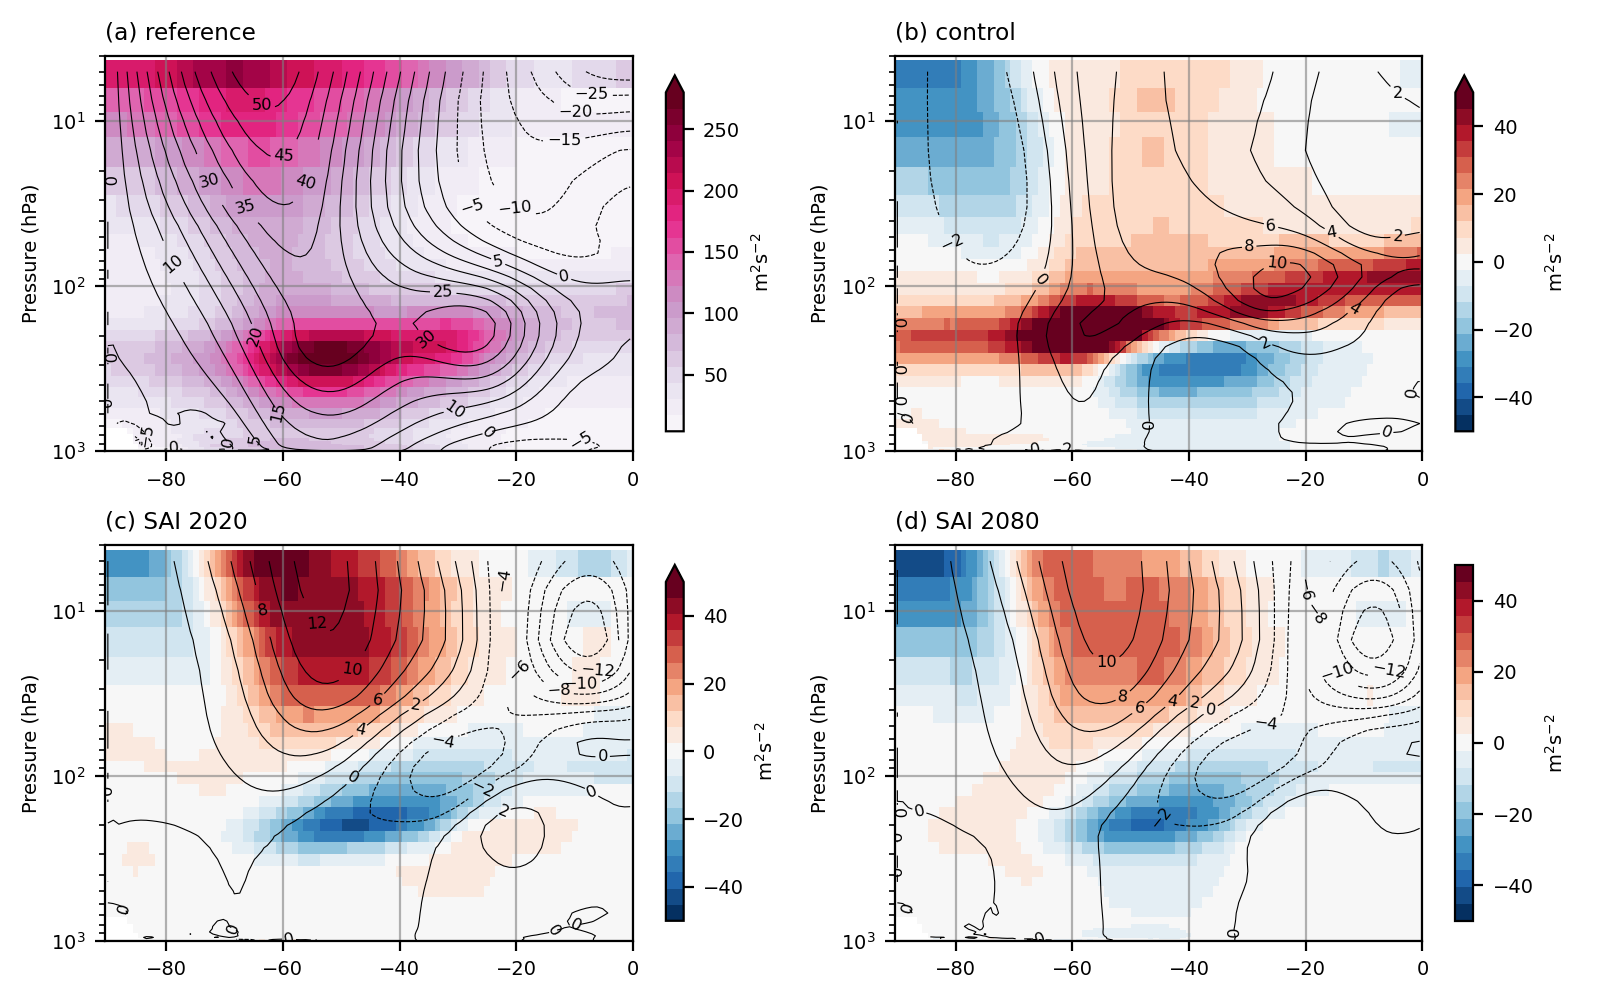
\includegraphics[width=\linewidth]{images/EKE_U_zmdiff_ann.png}
    \caption{Zonal mean difference EKE in m$^2$/s$^2$ (shading) and zonal mean difference zonal wind (contours) in intervals of 5 m/s, annual mean for reference 2020-2039 and all scenarios 2111-2130 compared to reference}
    \label{fig:EKE_U_zmdiff_ann}
\end{figure}

